% HEADER
\documentclass[class=article, crop=false]{standalone}
\usepackage{00_Preamble/frr_preamble}

% Packages
\usepackage{titlesec}
\usepackage{hyperref}
\usepackage{float}
\usepackage{graphics}
\usepackage{placeins}
\usepackage{adjustbox}
% END HEADER

\begin{document}
	\subsection{Final Design}
	\label{subsec:final-design}
	
	After the preliminary design was completed, several design iterations were made as the CAD assembly was further developed and specific parts were selected. Changes were made to resolve size constraint issues, reduce fabrication time, and reduce system cost. The final CAD assembly of the robot is presented in Figure \ref{fig:final-cad}.
	
	\FloatBarrier
	\begin{figure}[h]
	\centering
	 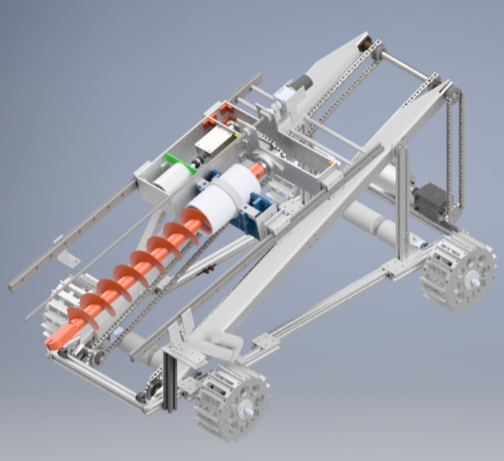
\includegraphics[width=0.6\linewidth]{09_Figures/final-cad.jpg}
	 \caption{Robot Controller flow diagram}
	 \label{fig:final-cad}
	\end{figure}
	\FloatBarrier
	
	\subsubsection{Frame Section}
	
	The frame was designed to be lightweight and simple to modify (Fig. 7). It was constructed from 30mm by 30mm aluminum extrusions connected by corner brackets and flat mounting plates. Two vertical supports near the back connect the conveyor. The motor and gearbox that drive the conveyor were placed on the back extrusion. Only minor length changes were made to the frame between the preliminary design review and the final design. The final weight was under 4 kg.
	
	\FloatBarrier
	\begin{figure}[h]
	\centering
	 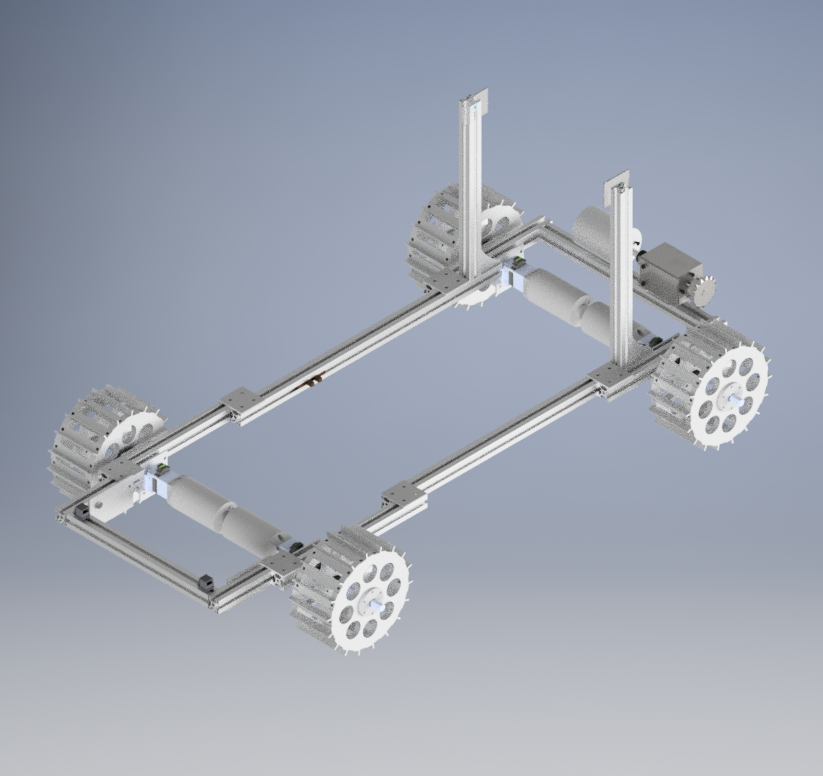
\includegraphics[width=0.6\linewidth]{09_Figures/frame-cad.jpg}
	 \caption{Robot Controller flow diagram}
	 \label{fig:final-cad}
	\end{figure}
	\FloatBarrier
	
	\subsubsection{Cost Budget}
	
	\subsubsection{Management Structure}
	Team members were distributed among three subgroups, mechanical, electrical, and programming, based on their area of interest and expertise. Members of each subteam were assigned to specific subsystems of the robot and worked in cross-disciplinary groups with other members from each subteam to fully design the subsystem. The purpose of the cross-functional groups was to ensure that all aspects of the design are considered simultaneously. Each of the subteams were managed by a subteam lead, whose responsibility was to allocate work and track progress for the design of their respective part of the robot. The subteam leads reported their progress to the team captain. The captain was responsible for tracking objectives, facilitating integration between various subteams, and ensuring that the high-level requirements are met.



	
	
	


	
\end{document}
